\documentclass[12pt]{article}

\usepackage{amsmath}
\usepackage[margin = 1in]{geometry}
\usepackage{booktabs}
\usepackage{natbib}
\usepackage{graphicx}
\usepackage{float}
\usepackage{setspace}
\usepackage{caption}
\captionsetup[table]{skip=10pt}
\usepackage[colorlinks=true, citecolor=blue]{hyperref}


\begin{document}


\begin{titlepage}
  \begin{center}
      \vspace*{1cm}
      \Huge
      \textbf{Analysis of Men's Tennis 2022 Grand Slam Performance}

      \large
      \vspace{0.5cm}
       Exploration of likelihood factors affecting Men's Tennis Grand Slam outcomes.
           
      \vspace{1.5cm}

      \textbf{Kaitlyn Shevlin}
     
      \vspace{0.8cm}
        
       \Large    
      Department of Statistics\\
      University of Connecticut\\
      Storrs, CT\\
           
  \end{center}
\end{titlepage}

\doublespace{}

\begin{abstract}

This research investigates the factors that lead to winning matches in Men's 
Singles Grand Slam tournaments. Utilizing data from 508 matches in 2022, 
the aim is to discover if ATP rankings of players is indicative of the outcome of 
match. In addition, match analysis will be conducted to explore singular factors 
such as court type, as well as a combination of factors such as if winning the 
first set will lead to a win. There is a lack of research on the accuracy of ATP 
ranking for the most recent year of play. This research will examine particular factors as well 
as new combinations of elements that affect the outcomes of major tournaments which 
aid predictive statistics for the next seasons as well as personal player performance 
analysis for improvement. We utilize logistic regression models to obtain results as well as graphics 
to depict the data. When performing the regression, the relationship between the 
opponents ATP ranking upon entering the match is significant, as well as the fourth 
round and quarter final round in predicting the outcome of the match as either an 
upset, meaning the lower ranked player wins the match, or as predicted, meaning the 
winner of the match having a higher ranking.\\


\noindent{\sc Keywords}:
Exploratory analysis; Sports Data; Statistics; Tennis Grand Slams.
\end{abstract}


\section{Introduction}
\label{sec:intro}

Tennis has a long and distinguished history, gaining popularity in
19th century France. The sport has developed into a world-class event
drawing a large fan base all across the world. The Men's Tennis Grandslam 
Tournaments are notorious events that feature the world's best tennis players. 
There are four Grand Slams- the Australian Open, the French Open, Wimbledon, 
and the U.S. Open, spanning from January to September. Extensive research has 
been completed on modeling future and past player performance in conjunction 
with the improvement of game tracking technologies.

The goal of tennis is to win enough points to win a game, and then enough games 
to win a set, and finally enough sets to win a match \citet{Ifttennis2021Grand}. 
The points go from 0 to 15, to 30, to 40 and then the next point wins. If both 
players are at 40, it is called a deuce and the person must win by two--it becomes 
40-deuce, and then if the leader is up and scores again, they win. If the score 
becomes tied again, it goes back to 40-40. To win a set, you must win six games. 
If it is 5-5, then a player must win by two. For most matches, the common format 
is the best three of five. 

Exploratory analysis about tennis is important for metrics on both the
courts and matches, as well as the players. Many predictions are made well 
before the Grand Slams are played, mainly based off analysis and trends. 
Looking at past ATP rankings of players going into the tournament, and then 
examining the outcome of the match, will reveal how ATP translates to the 
matches and if the player with the higher ATP ranking going into the match 
is more likely to win.

Prior research has been done regarding top ranked tennis players, both males and 
females. Much analysis surrounding top performers throughout the years and the 
relationshp between the changes in ATP rankings have been researched. As this 
dataset includes statistics from 2022, there is less specific research conducted.

Tennis is unique in that several court surfaces are used- clay, grass, and hard 
surfaces, that players must adapt to. Each court type has various advantages and
disadvantages around play and maintence, in addition to player specific preferences.
The French open is played on clay courts which can be characterized by high bounce
but overall a slow surface which is best for baseline players. Rafael Nadal is 
considered "the King of Clay," which can be attributed to him growing up in Spain
where clay courts are predominant. His specific skillset also aligns well with the
features of clay courts \citet{Jurejko2018French}. Wimbledon takes place on grass 
courts which are the opposite to clay, in that it is the fastest surface with a low bounce. 
Roger Federer excelled here as it favors players with large serves and those who prefer to play close to the
net. Hard courts are utilzed for the U.S. and Australian Opens, characterized by high,
predictable bounces and medium speed \citet{Schwartz1977The}. 

\citet{Pollard2006} investigated the four Grand Slam Men's Singles data for Lack of 
independence of set outcomes by examining the frequencies of categories to see the 
probability of winning a set within a match. His analysis looked at data over a span of 
ten years and found that winning varies from set to set, and that the better player tends 
to elevate his play in some situations, although they may not be the winner.

The Association of Tennis Professionals (ATP) is the world's governing
body for men's tennis whereas the Women's Tennis Associaton (WTA)
is the world's governing body in women's tennis. Both the ATP and
WTA have computerized tennis rankings for singles and doubles players.
There is no systematic ranking for mixed doubles as of yet. These
rankings are based on points earned in one's best 19 events, 16 for women,
as this number is capped at 19 to prevent someone who plays in more tournaments
per year to be at an advantage. Points awarded for Grand Slams are greater
than points for other tournaments and events \citet{Nag2022Tennis}.

The following table shows the ATP ranking points awarded for each type of match.

\begin{table}[ht]
  \caption{ATP ranking points table}
  \label{tab:ATP}
\centering
\begin{tabular}{
  |p{\dimexpr.285\linewidth-2\tabcolsep-1.3333\arrayrulewidth}
  |p{\dimexpr.065\linewidth-2\tabcolsep-1.3333\arrayrulewidth}
  |p{\dimexpr.065\linewidth-2\tabcolsep-1.3333\arrayrulewidth}
  |p{\dimexpr.065\linewidth-2\tabcolsep-1.3333\arrayrulewidth}
  |p{\dimexpr.065\linewidth-2\tabcolsep-1.3333\arrayrulewidth}
  |p{\dimexpr.065\linewidth-2\tabcolsep-1.3333\arrayrulewidth}
  |p{\dimexpr.065\linewidth-2\tabcolsep-1.3333\arrayrulewidth}
  |p{\dimexpr.065\linewidth-2\tabcolsep-1.3333\arrayrulewidth}
  |p{\dimexpr.065\linewidth-2\tabcolsep-1.3333\arrayrulewidth}
  |p{\dimexpr.065\linewidth-2\tabcolsep-1.3333\arrayrulewidth}
  |p{\dimexpr.065\linewidth-2\tabcolsep-1.3333\arrayrulewidth}
  |p{\dimexpr.065\linewidth-2\tabcolsep-1.3333\arrayrulewidth}|
  }
  \hline
Tournament Level & W & F & SF & QF & R16 & R32 & R64 & R128 & Q & Q3 & Q2\\ 
  \hline
Grand Slam & 2000 & 1200 & 720 & 360 & 180 & 90 & 45 & 10 & 25 & 16 & 8 \\ 
\hline
ATP 1000 - 96 Draw & 1000 & 600 & 360 & 180 & 90 & 45 & 25 & 10 & 16 &  & 8\\ 
\hline
ATP 1000 - 48/56 Draw & 1000 & 600 & 360 & 180 & 90 & 45 & 10 &  & 25 &  & 16\\
\hline
ATP 500 - 48 Draw & 500 & 300 & 180 & 90 & 45 & 20 &  &  & 10 &  & 4\\ 
\hline
ATP 500 - 32 Draw & 500 & 300 & 180 & 90 & 45 &  &  &  & 20 &  & 10\\ 
\hline
ATP 250 - 48 Draw & 250 & 150 & 90 & 45 & 20 & 10 &  &  & 5 &  & 3\\
\hline
ATP 250 - 32 Draw & 250 & 150 & 90 & 45 & 20 &  &  &  & 12 &  & 6\\
\hline
ATP Challenger Tour 125 & 125 & 75 & 45 & 25 & 10 & & & & & & \\
\hline
ATP Challenger Tour 110 & 110 & 65 & 40 & 20 & 9 & 5 & & & & & \\
\hline
ATP Challenger Tour 100 & 100 & 60 & 35 & 18 & 8 & 5 & & & & & \\
\hline
ATP Challenger Tour 90 & 90 & 55 & 33 & 17 & 8 & 5 & & & & & \\
\hline
ATP Challenger Tour 80 & 80 & 48 & 29 & 15 & 7 & 3 & & & & & \\
\hline
ITF World Tennis Tour $25,000 / $25,000+H & 20 & 12 & 6 & 3 & 1 & & & & & & \\
\hline
ITF World Tennis Tour $15,000 / $15,000+H & 10 & 6 & 4 & 2 & 1 & & & & & & \\
  \hline
\end{tabular}
\end{table} 


This goal of this research is to investigate if ATP is a significant factor
in predicting the outcome of the match. Prior research has revealed weaknesses 
in the ATP ranking system which has its basis rooted in points. Other ranking 
systems such as UTR, do not deal with points, instead it utilizes algorithms to 
assess player performance in relation to their most recent matches \citet{Bodo2022Rankings}. 
Keeping this in mind, this exploration will see how heavily and accurately ATP 
ranking played a role in the outcome of the match in addition to other variables 
including court surface, and if winning the first set is notable.



\section{Data}
\label{sec:data}

The data is acquired from tennis.data.co.uk which provides detailed historical 
and recent sports data \citep{TennisBetting}. The site compiles the information 
from the sources ATPtennis.com, ATP Tour Rankings and Results Page, and Sony 
Ericsson WTA Tour. The dataset for this research includes figures from the four 
men's tennis Grand Slam tournaments in 2022. The data provides many specific 
factors that play a role in matches as well as an abundance of results which will 
aid in the analysis and regression.

There are missing values in W4, L4, W5, L5, due to the fact that the matches are 
best three out of five, meaning that a player can win in three or four sets and 
not have to play the additional sets. 

The element descriptions are clearly labeled on the site as follows: 

ATP = tournament number for men

WTA = tournament number for women

Location = venue of tournament

Tournament =  name of tournament (four major Grand Slams)

Series = name of ATP tennis series

Court = type of court (indoors or outdoors)

Surface = type of surface (clay, hard, carpet, or grass)

Round = round of match

Best of = maximum number of sets playable in a match (5 for mens) 

Winner = match winner 

Loser = match loser

WRank = ATP entry ranking of match winner as of the start of the tournament

LRank = ATP entry ranking of match loser as of the start of the tournament

WPts = ATP entry points of match winner as of the start of the tournament

LPts = ATP entry points of match loser as of the start of the tournament

W1 = number of games won in 1st set by match winner

L1 = number of games won in 1st set by match loser

W2 = number of games won in 2nd set by match winner

L2 = number of games won in 2nd set by match loser

W3 = number of games won in 3rd set by match winner

L3 = number of games won in 3rd set by match loser

W4 = number of games won in 4th set by match winner

L4 = number of games won in 4th set by match loser

W5 = number of games won in 5th set by match winner

L5 = number of games won in 5th set by match loser

Wsets = number of sets won by match winner

Lsets = number of sets won by match loser

Comment = comment on the match (completed, won through retirement of loser, or walkover)\\

The data provides number of games won in each set for match winner and loser, which will 
aid in the examination of predicting match winner by success in the first game as well 
as the relationships between ATP ranking of the players coming into the match and the outcome 
of the match. No visualizations are provided but clear descriptives are stated.


\section{Methods}
\label{sec:meth}


I will be using logistic regression which is a classification algorithm. The logistic 
function is
\begin{equation}
  \label{eq:logreg}
    \ \sigma(t) = \frac{1}{1 + e^-t}
\end{equation}
 
This equation sets up for predictive analysis to describe the relationship between 
one dependent variable and one or more independent variables. It allows for the output 
to be explicated as a probability from 0 to 1.
  
The logistic regression for the prediction of the match outcome as either an upset or as predicted 
consists of a vector of n match variables $x = (x_1, x_2,..., x_n)$ with parameters $\beta = (\beta_0,
\beta_1,...,\beta_n)$. This model can then be used to make a prediction by projecting a point in 
the n-dimensional space to a real number:
\begin{equation}
  \label{eq:logreg}
    \ z = \beta_0 + \beta_1 x_1 + \beta_2 x_2 + ... + \beta_nx_n
\end{equation}

The regression will explore the relationships between factors as well as interactions 
between factors such as WRank and LRank to find out if coming into the match with a 
better ranking is indicative of the outcome. The dependent variable is the match outcome 
which is listed as either an upset or as predicted.

The parameter estimates show the change in the response variable associated with a change in one 
unit of the parameter, with all the other predictors held constant. We are conducting the regression 
analysis under the assumptions of linearity, independence, normality, and homoscedasticity. In 
addition, we have to assume that the data is recorded correctly. For theoretical claims, we operate 
under the assumping that a measurement is capturing something significant.

\begin{figure} [htbp]
  \centering
  \includegraphics[width=\textwidth, scale=0.5]{assumptions.pdf}
  \caption{Assumptions for the regression model.}
 \label{fig:assumptions}
\end{figure}

The residuals vs. fitted graph show random spread with no patterns around the horizontal line, 
showing a linear relationship. The normal Q-Q plot checks the normality of residuals which follow the 
straight line, meeting the normality assumption. The scale location graph checks the homoscedasticity, 
and the graph follows no patterns and is random around the horizontal line, satisfying the assumption. 
For the residuals vs. leverage graph, it appears to be independent. These graphs provide proof of the 
satisfaction of all the assumptions. 


\section{Application}
\label{sec:application}

The winners of the four Grand Slams in 2022 are below. Many of the names are familiar 
as they are well-renowned players and their rankings going into the final matches were 
all in the top 5.

\begin{table}[ht]
  \caption{Winners of the four Grand Slams}
  \label{tab:winner}
\centering
\begin{tabular}{rrr}
  \hline
Winner & Tournament & Ranking\\
  \hline
Rafael Nadal & Australian Open & 5\\
Rafael Nadal & French Open & 5\\
Novak Djokovic & Wimbledon & 3\\
Carlos Alcaraz & US Open & 4\\
  \hline
\end{tabular}
\end{table}


To find if the ATP ranking of the players entering the match have an impact, I created a new 
variable called upset which gives the output "Predicted" if the winner of the match had a higher 
ATP ranking coming in; and "Upset" if the loser of the match had the higher ranking. The graph 
below shows the count of each.

\begin{table}[! h]
  \caption{Count of Outcome}
  \label{tab:upset}
\centering
\begin{tabular}{rr}
  \hline
Outcome & Count \\
  \hline
Predicted & 141 \\
Upset & 367 \\
  \hline
\end{tabular}
\end{table}


As seen in the table above, many upsets occur, leading us at first glance to believe that ATP 
ranking is not a good predictor. This coincides with the numbers found in: 


\begin{figure} [! h]
  \centering
  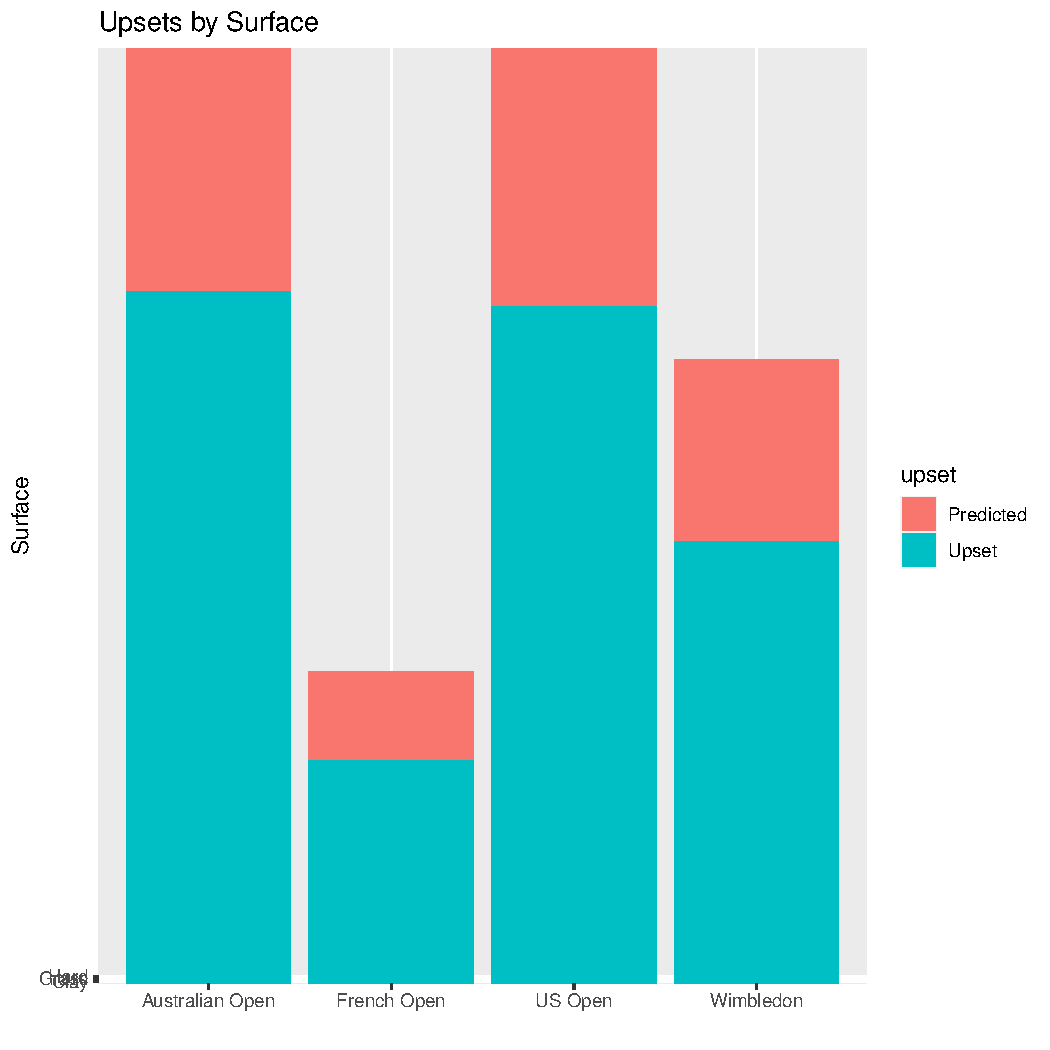
\includegraphics[width=\textwidth, scale=0.5]{surfaceoutcome.pdf}
  \caption{Outcomes by Surface.}
 \label{fig:surfaceupsets}
\end{figure}

The figure above shows that the majority of all matches, on every court type, are upsets. This 
is another indicator that ATP ranking is not accurate in predicting the outcome of the match. 
The visual allows for a clear view of the scale of the amount of upsets over predicted outcomes.


\begin{figure} [! h]
  \centering
  \includegraphics[width=\textwidth, scale=0.5]{rankoutcome.pdf}
  \caption{Outcomes by Rank.}
 \label{fig:rankoutcome}
\end{figure}

Figure[~\ref{fig:rankoutcome}] shows the relationship between the winner's ranking and the loser's 
ranking coming into the match and the subsequent outcome of the match. The graph shows that 
typically the higher the winner is ranked coming into the match, the more likely they won 
the match. Where the rankings are pretty even going into the match, there are a lot of upsets. 
This could explain the large number of upsets seen in table[~\ref{tab:upset}] and figure[~\ref{fig:surfaceupsets}].


Summary statistics for the model are as follows:

\begin{figure} [! h]
  \centering
  \includegraphics[width=\textwidth, scale=0.25]{logreg.pdf}
  \caption{This figure shows the output of the model from R.}
 \label{fig:logreg}
\end{figure}

From the output, we see that the model has a Multiple R-Squared value of 0.52, which indicates 
that 52\% of the variance is explained by the model. This is a relatively good model, however, 
it could be improved by including other variables that impact the match. For this analysis, we 
are only testing for these specific variables seen in the model.

The results of the logistic regression show that WRank, the relationship between WRank and LRank, 
4th Round, and the Quarter final round are significant variables in predicting the outcome of the 
match at the significance level of 0. Surface type--grass and hard--were not significant, along 
with the second round, third round, semifinals, the final, W1, L1, LRank, and the relationship 
between W1 and L1.




\section{Discussion}
\label{sec:discussion}

The results of the logisitic regression shows that there is a relationship between the rankings of 
the players coming into the match, but it may not be in the direction that one would assume. 
Based on Table[~\ref{tab:upset}], Figure[~\ref{fig:surfaceupsets}], and Figure[~\ref{fig:rankoutcome}],
there appear to be more upsets than predicted outcomes. These graphs, in accordance with Figure[~\ref{fig:logreg}],
show a negative relationship between WRank and LRank, meaning that coming into the tournament with a higher 
ranking does not mean that you are going to win the match in a lot of cases. There seems to be no relationship 
between winning the first set, as well as court type with the outcome of the match. With additional information 
and factors added, we may see that these insignificant factors in this model are significant in another model 
due to a player's preferences, however, this dataset only includes statistics from the matches and not player's background.

Some limitations of this dataset include the fact that the data is solely based on the match  
and the numbers from match being played. It could be a stronger model by including variables 
based on the players, such as dominant hand, number of hours practiced, and court type they 
practice on. These additional variables could influence the outcome of matches. This current 
study is only utilizing data from 2022 so for future studies, a wider variety of newer data 
can be used to further analyze trends and changes over time.

The main contributions of this study are to show that ATP ranking is not completely accurate 
or a good predictor of the outcome of Men's Grand Slam tennis matches. It is worth pursuing 
further analysis and exploration of other ranking systems that accurately portray a player's 
standings and a way to improve upon ATP's points focused approach.

Future research around this topic of accuracy of ATP ranking, and the combinations of variables 
that lead to a winner of the men's Grand Slam titles can be vastly explored. If more research is done to 
uncover that ATP ranking is not the best and most accurate calculation to represent a player's 
statistics, then a new measurement may be instituted as the one most widely used. Or, the ATP 
ranking can adjust to include additional factors that make it more precise and informative. 



\bibliography{references}
\bibliographystyle{chicago}

\end{document}